\documentclass{article} % For LaTeX2e
\usepackage{nips14submit_e,times}
\usepackage{hyperref}
\usepackage{url}
\usepackage{graphicx}
\usepackage{amsmath}
\usepackage{caption}
\usepackage{subcaption}
%\documentstyle[nips14submit_09,times,art10]{article} % For LaTeX 2.09


\title{Learning together: Preventing co-adaptation and promoting variance in neural network ensembles}


\author{
Derek Racine \\
Department of Computer Science \\
Dartmouth College\\
Hanover, NH 03755 \\
\texttt{derek.r.racine.14@dartmouth.edu} \\
\And
Phillip Coletti\\
Thayer School of Engineering\\
Dartmouth College\\
Hanover, NH 03755 \\
\texttt{phillip.m.coletti.14@dartmouth.edu} \\
}

% The \author macro works with any number of authors. There are two commands
% used to separate the names and addresses of multiple authors: \And and \AND.
%
% Using \And between authors leaves it to \LaTeX{} to determine where to break
% the lines. Using \AND forces a linebreak at that point. So, if \LaTeX{}
% puts 3 of 4 authors names on the first line, and the last on the second
% line, try using \AND instead of \And before the third author name.

% \newcommand{\fix}{\marginpar{FIX}}
% \newcommand{\new}{\marginpar{NEW}}

\nipsfinalcopy % Uncomment for camera-ready version

\begin{document}


\maketitle

% \begin{abstract}
% The abstract paragraph should be indented 1/2~inch (3~picas) on both left and
% right-hand margins. Use 10~point type, with a vertical spacing of 11~points.
% The word \textbf{Abstract} must be centered, bold, and in point size 12. Two
% line spaces precede the abstract. The abstract must be limited to one
% paragraph.
% \end{abstract}

\section{Project motivation}

\subsection{Introduction}

In practice, regularizing complex models to prevent overfitting often works better than using simpler ones, which risk underfitting. Deep neural networks (DNNs) have an enormous capacity for learning because they can have a large number of layers and hidden units. However, with millions of parameters, these networks are prone to overfit even very large datasets. As a result, a wide range of techniques have been developed to regularize neural networks, such as early stopping and weight elimination (Weigend et al., 1991) [1].

Recently, Hinton et al. proposed a new form of regularization called Dropout (Hinton et al., 2012) [2]. For each training example, some percentage of the input or hidden units are randomly omitted per layer. The resulting error is then backpropagated only through the remaining activations. This method prevents co-adaptations in which a feature detector is only helpful in the context of specific other feature detectors. That is, the feature detectors would otherwise be tuned to work well together on the training data but not on the test data. Thus, Dropout helps prevent overfitting, leading to better generalization performance (See Figure 1).

\begin{figure}[h!]
\begin{center}
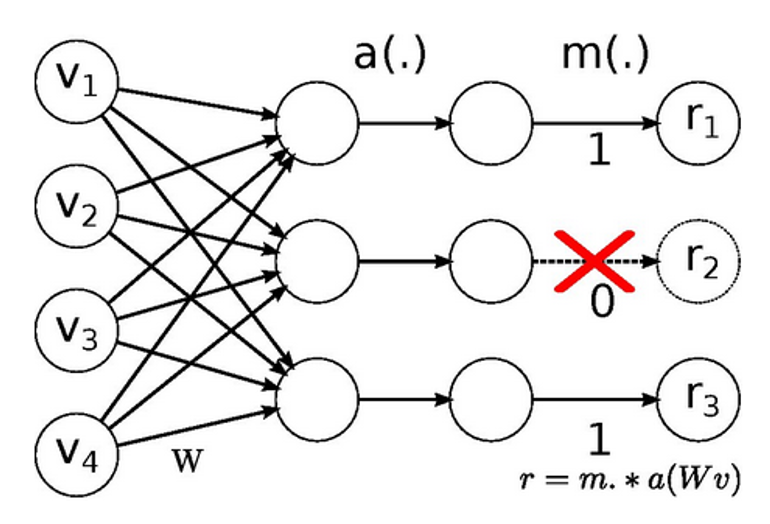
\includegraphics[width=300pt]{Dropout_Figure.png}
\caption{In Dropout, a random subset of units in every layer (including the input layer) are set to 0 for each training example. The resulting error is then backpropagated only through the remaining units.}
\end{center}
\end{figure}

While Dropout is applied during finetuning, unsupervised pretraining has also been shown to act as a regularizer (Erhan et al., 2010) [3]. Specifically, pretraining initializes the network to a part of weight space where there are fewer basins of attraction that are reachable through gradient descent with backpropagation. Pretraining and Dropout can be combined to yield state-of-the-art accuracy on several datasets, including MNIST and CIFAR-10 (0.21\% and 9.32\%, respectively; Wan et al., 2013). In this case, pretraining is done via greedy, layer-wise learning of Restricted Boltzmann Machines (RBMs). RBMs are inherently stochastic in that hidden units are turned on (set to 1) with probability equal to their activations, or the output of the sigmoid function applied to the sum of their inputs (including a bias term).

\begin{figure}[h!]
\begin{center}
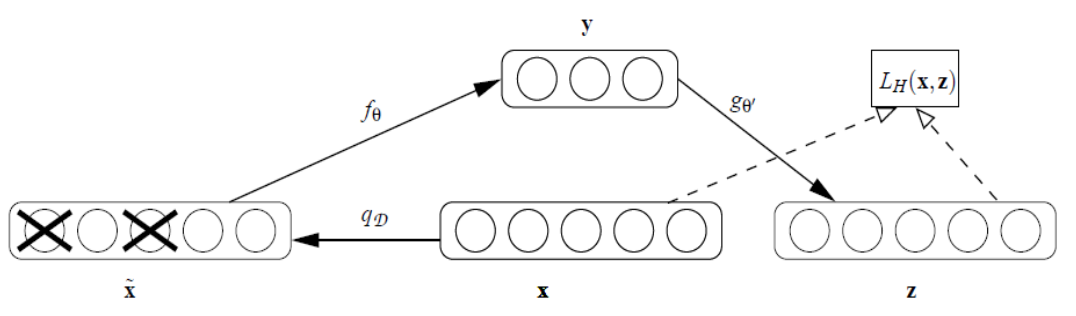
\includegraphics[width=300pt]{SDAE_Figure.png}
\caption{Each layer in a stacked denoising autoencoder is trained to reconstruct the original input from a corrupted version of it, in which a random subset of the values have been set to 0.}
\end{center}
\end{figure}

Vincent et al. (2008) introduced an alternative form of pretraining that also has a random component: stacked denoising autoencoders (SDAEs) [6]. Each hidden layer is trained to reconstruct either the visible or hidden units of the layer before it like a basic autoencoder, except that a random subset of the inputs are corrupted (set to 0, in this paper). Importantly, the error objective is still to reproduce the original (uncorrupted) input. By forcing a layer to be robust to partial destruction of the input, it captures features that represent more stable structures (in terms of dependencies and regularities) in the distribution of the data. In other words, the model has to learn the relationship between the missing (corrupted) inputs and the remaining values in order to reconstruct them (See Figure 2). Qualitatively, the filters (features) learned on the MNIST handwritten digit set using SDAEs are much more distinctive than those found using basic autoencoders. In particular, they encode local blobs or strokes rather than nearly uniform grey patches.

\subsection{Types of Corruption}

A natural question that arises from these studies is whether different types of corruption will yield the same results. Indeed, Vincent et al. (2010) explored this idea with SDAEs and found that some forms of corruption perform better than others [4]. Moreover, they learn qualitatively different features. For example, salt-and-pepper noise results in Gabor-like filters, whereas zero-masking noise produces filters that look like oriented gratings (See Figure 3). Between these and Gaussian noise, salt-and-pepper noise results in the lowest classification error.

\begin{figure}
\centering
\begin{subfigure}{.5\textwidth}
  \centering
  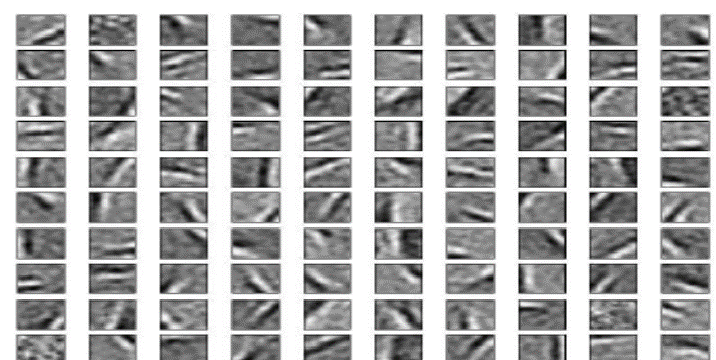
\includegraphics[width=150pt]{SDAE_Filters_SaltAndPepperNoise.png}
  \caption{Filters learned with salt-and-pepper noise.}
  \label{fig:sub1}
\end{subfigure}%
\begin{subfigure}{.5\textwidth}
  \centering
  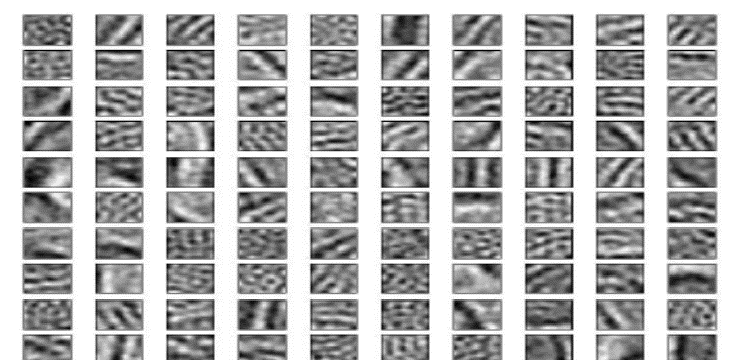
\includegraphics[width=150pt]{SDAE_Filters_ZeroMasking.png}
  \caption{Filters learned with zero-masking.}
  \label{fig:sub2}
\end{subfigure}
\caption{Features learned in the first hidden layer (filters) on the MNIST handwritten digit set.}
\label{fig:test}
\end{figure}

Interestingly, the Dropout technique shares many characteristics with training SDAEs. In practice, both techniques involve setting some number of the (input or hidden) units in every layer to 0. From a theoretical perspective, they both force the model to learn about the distribution underlying the data without being able to rely on having complete information. In order to make up for these lost values, the network captures deeper structures that can explain how the inputs relate to each other. Such regularities are more likely to be representative of the data distribution, and therefore generalize well to new examples at test time. While different types of corruption have been tested in the context of SDAEs, they have not been in Dropout. Therefore, we would propose to explore different types corruptions in Dropout to see if it improves performance, as it did with SDAEs.

\subsection{Ensemble Learning}

Wan et al. (2013) recently generalized Dropout to DropConnect, where random subsets of weights in each layer are dropped instead of entire units [5]. However, this change does not lead to substantial improvements. That said, an interesting result of their study was that averaging multiple models gave significantly better overall performance. Model voting works because the prediction error of the ensemble (by aggregating the votes of all models) is at worst equal to the average of the error of each individual model predicting in isolation.

Random forests are a more thoroughly studied application of ensemble learning. A random forest can be grown without risk of overfitting. As the number of trees in the forest increases, the variance of the ensemble prediction decreases without increasing the bias. Thus, the prediction becomes more accurate as the ensemble size is increased. However, the performance is saturated beyond a certain threshold (See Figure 4). Fundamentally driving the performance of random forests (and by extension, ensemble learning algorithms in general), is the predictive strength of the individual models within the forest and the variance between these models predictions. That is, different models are better at predicting different classes leading to overall improvement when these predictions are combined.

\begin{equation*}
	Generalization Error = \frac{correlation}{strength}
\end{equation*}

\begin{figure}[h!]
\begin{center}
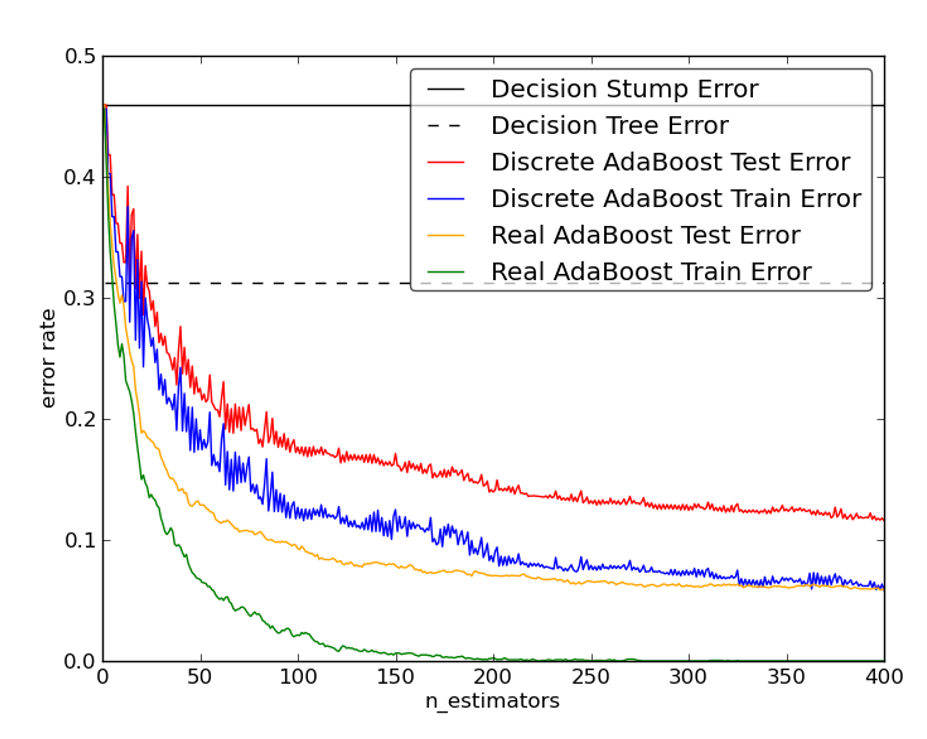
\includegraphics[width=300pt]{RandomForest_Graph.png}
\caption{As the number of estimators or trees in the forest increases (regardless of the model), the error of the overall prediction decreases, although it eventually saturates.}
\end{center}
\end{figure}

Thus, the generalization error of an ensemble can be improved by increasing the variance between the model predictions or by increasing the variance between the models. In a random forest, each individual tree is a worse predictor than a deterministic decision tree trained on the full data. However, the variance between the models allows the ensemble to be a far more accurate predictor. The trees learn different subtle nonlinearities within the data and become very good at predicting certain classes very well when certain combinations of inputs are present. Thus, for any given example, a small subset of trees in the forest will be very good predictors, with the remainder of the forest averaging out to random noise.

\section{Experiments}

First, we plan to implement Dropout using the architecture described in Wan et al. (2013) in order reproduce their results. Note that their model includes a 2-layer convolutional neural network feature extractor as a preprocessing step. Second, we will experiment with different types of corruption: specifically, zero-masking (benchmark), salt-and-pepper noise, Gaussian noise, and random values in the range of the input data (so [0,1] for hidden units). Third, we are going to explore model averaging in the context of corruption. In particular, we plan to vary the types of corruption and the rate of dropout within ensembles (as well as test different voting schemes). Our hypothesis is that by encouraging each individual model to learn different sets of features (increasing the variance), the overall prediction will be better.

\subsection{Datasets}

The datasets we plan to use are the MNIST handwritten digit set in order to compare our results to known benchmarks and the CIFAR-10 data set to see if we can make more significant improvements on a more realistic, less saturated problem. These data sets can be obtained online from \url{http://yann.lecun.com/exdb/mnist/} and \url{http://www.cs.toronto.edu/~kriz/cifar.html}, respectively.

\begin{figure}
\centering
\begin{subfigure}{.5\textwidth}
  \centering
  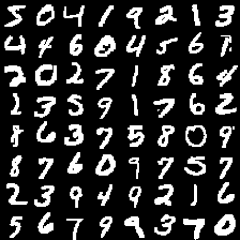
\includegraphics[width=150pt]{MNIST_Image.png}
  \caption{Examples from the MNIST handwritten digit set.}
  \label{fig:sub1}
\end{subfigure}%
\begin{subfigure}{.5\textwidth}
  \centering
  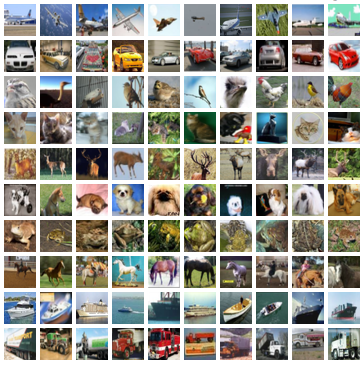
\includegraphics[width=150pt]{CIFAR-10_Image.png}
  \caption{Example images from the CIFAR-10 data set}
  \label{fig:sub2}
\end{subfigure}
\caption{Examples from the two data sets we plan on using.}
\label{fig:test}
\end{figure}

\subsection{Baselines}

We plan on using the results obtained in Wan et al. (2013) using Dropout and model averaging on the MNIST and CIFAR-10 data sets as baselines to which we can compare our performance.

\section{Milestone}

By our milestone, we expect to have implemented the Dropout model and tested all the different types of corruption on the MNIST and CIFAR-10 data sets. Before the final due date, we will have explored how corruption can be varied within the context of ensemble learning to yield better results.

% \section{General formatting instructions}
% \label{gen_inst}

% The text must be confined within a rectangle 5.5~inches (33~picas) wide and
% 9~inches (54~picas) long. The left margin is 1.5~inch (9~picas).
% Use 10~point type with a vertical spacing of 11~points. Times New Roman is the
% preferred typeface throughout. Paragraphs are separated by 1/2~line space,
% with no indentation.

% Paper title is 17~point, initial caps/lower case, bold, centered between
% 2~horizontal rules. Top rule is 4~points thick and bottom rule is 1~point
% thick. Allow 1/4~inch space above and below title to rules. All pages should
% start at 1~inch (6~picas) from the top of the page.

% %The version of the paper submitted for review should have ``Anonymous Author(s)'' as the author of the paper.

% For the final version, authors' names are
% set in boldface, and each name is centered above the corresponding
% address. The lead author's name is to be listed first (left-most), and
% the co-authors' names (if different address) are set to follow. If
% there is only one co-author, list both author and co-author side by side.

% Please pay special attention to the instructions in section \ref{others}
% regarding figures, tables, acknowledgments, and references.

% \section{Headings: first level}
% \label{headings}

% First level headings are lower case (except for first word and proper nouns),
% flush left, bold and in point size 12. One line space before the first level
% heading and 1/2~line space after the first level heading.

% \subsection{Headings: second level}

% Second level headings are lower case (except for first word and proper nouns),
% flush left, bold and in point size 10. One line space before the second level
% heading and 1/2~line space after the second level heading.

% \subsubsection{Headings: third level}

% Third level headings are lower case (except for first word and proper nouns),
% flush left, bold and in point size 10. One line space before the third level
% heading and 1/2~line space after the third level heading.

% \section{Citations, figures, tables, references}
% \label{others}

% These instructions apply to everyone, regardless of the formatter being used.

% \subsection{Citations within the text}

% Citations within the text should be numbered consecutively. The corresponding
% number is to appear enclosed in square brackets, such as [1] or [2]-[5]. The
% corresponding references are to be listed in the same order at the end of the
% paper, in the \textbf{References} section. (Note: the standard
% \textsc{Bib\TeX} style \texttt{unsrt} produces this.) As to the format of the
% references themselves, any style is acceptable as long as it is used
% consistently.

% As submission is double blind, refer to your own published work in the 
% third person. That is, use ``In the previous work of Jones et al.\ [4]'',
% not ``In our previous work [4]''. If you cite your other papers that
% are not widely available (e.g.\ a journal paper under review), use
% anonymous author names in the citation, e.g.\ an author of the
% form ``A.\ Anonymous''. 


% \subsection{Footnotes}

% Indicate footnotes with a number\footnote{Sample of the first footnote} in the
% text. Place the footnotes at the bottom of the page on which they appear.
% Precede the footnote with a horizontal rule of 2~inches
% (12~picas).\footnote{Sample of the second footnote}

% \subsection{Figures}

% All artwork must be neat, clean, and legible. Lines should be dark
% enough for purposes of reproduction; art work should not be
% hand-drawn. The figure number and caption always appear after the
% figure. Place one line space before the figure caption, and one line
% space after the figure. The figure caption is lower case (except for
% first word and proper nouns); figures are numbered consecutively.

% Make sure the figure caption does not get separated from the figure.
% Leave sufficient space to avoid splitting the figure and figure caption.

% You may use color figures. 
% However, it is best for the
% figure captions and the paper body to make sense if the paper is printed
% either in black/white or in color.
% \begin{figure}[h]
% \begin{center}
% %\framebox[4.0in]{$\;$}
% \fbox{\rule[-.5cm]{0cm}{4cm} \rule[-.5cm]{4cm}{0cm}}
% \end{center}
% \caption{Sample figure caption.}
% \end{figure}

% \subsection{Tables}

% All tables must be centered, neat, clean and legible. Do not use hand-drawn
% tables. The table number and title always appear before the table. See
% Table~\ref{sample-table}.

% Place one line space before the table title, one line space after the table
% title, and one line space after the table. The table title must be lower case
% (except for first word and proper nouns); tables are numbered consecutively.

% \begin{table}[t]
% \caption{Sample table title}
% \label{sample-table}
% \begin{center}
% \begin{tabular}{ll}
% \multicolumn{1}{c}{\bf PART}  &\multicolumn{1}{c}{\bf DESCRIPTION}
% \\ \hline \\
% Dendrite         &Input terminal \\
% Axon             &Output terminal \\
% Soma             &Cell body (contains cell nucleus) \\
% \end{tabular}
% \end{center}
% \end{table}

\newpage
\begin{thebibliography}{30}

\bibitem{cite1} A. S. Weigend, D. E. Rumelhart, and B. A. Huberman.
Generalization by weight-elimination with applica-
tion to forecasting. In NIPS, 1991.

\bibitem{cite2} G. E. Hinton, N. Srivastava, A. Krizhevsky,
I. Sutskever, and R. Salakhutdinov. Improving neu-
ral networks by preventing co-adaptation of feature
detectors. CoRR, abs/1207.0580, 2012.

\bibitem{cite3} D. Erhan, A. Courville, Y. Bengio, and P. Vincent. Why does unsupervised pre-training help deep learning? In Proc. AISTATS '10, May 2010, vol. 9, pp. 201-208.

\bibitem{cite4} P. Vincent, H. Larochelle, I. Lajoie, Y. Bengio, and P.-A. Manzagol, “Stacked 
denoising autoencoders: learning useful representations in a deep network with a 
local denoising criterion,” J. Mach. Learn. Res., vol. 11, no. 11, pp. 3371–3408, 
2010.

\bibitem{cite5}  Li Wan, Matthew Zeiler, Sixin Zhang, Yann L Cun, and Rob Fergus. Regularization of neural
networks using dropconnect. In International Conference on Machine Learning, 2013.

\bibitem{cite6}Vincent, Pascal, et al. "Extracting and composing robust features with denoising autoencoders." Proceedings of the 25th international conference on Machine learning. ACM, 2008.

\end{thebibliography}

\end{document}